\section{Dual-Learning Fault Localization}
\label{sec:dual-learning}

\begin{figure}[t]
	\centering
	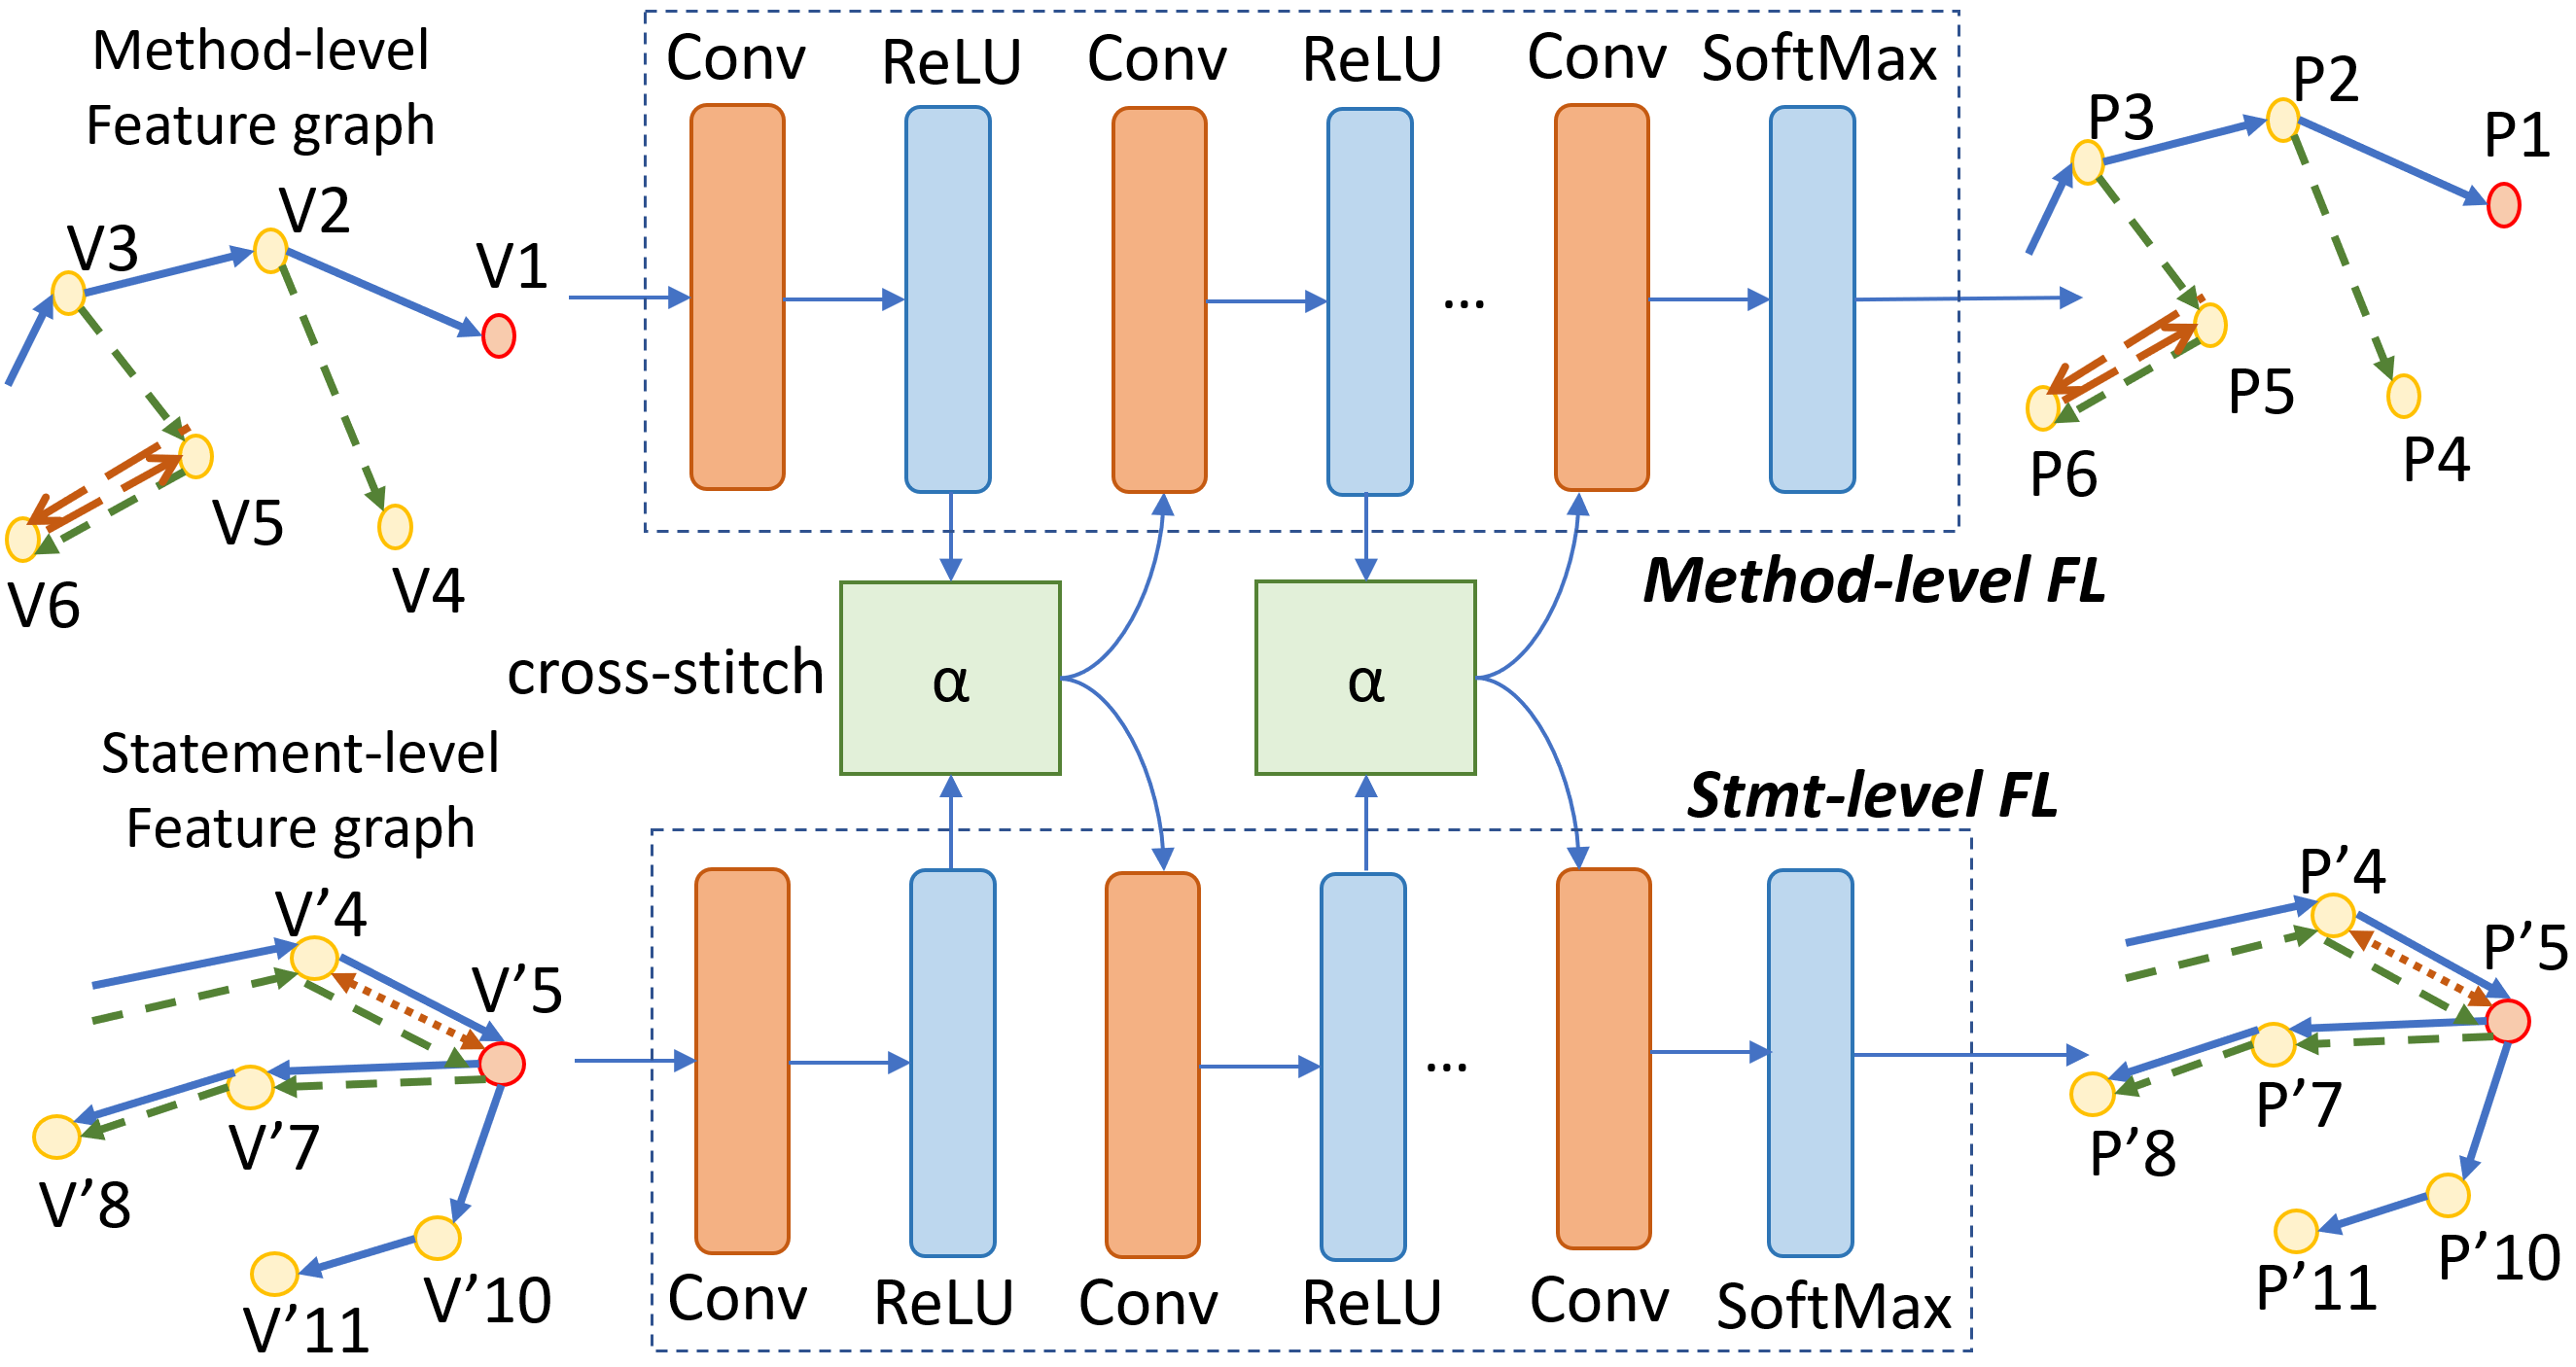
\includegraphics[width=3.4in]{graphs/dual-learning.png}
	\caption{Dual-Learning Fault Localization}
	\label{dual-learning}
\end{figure}

\begin{figure}[t]
	\centering
	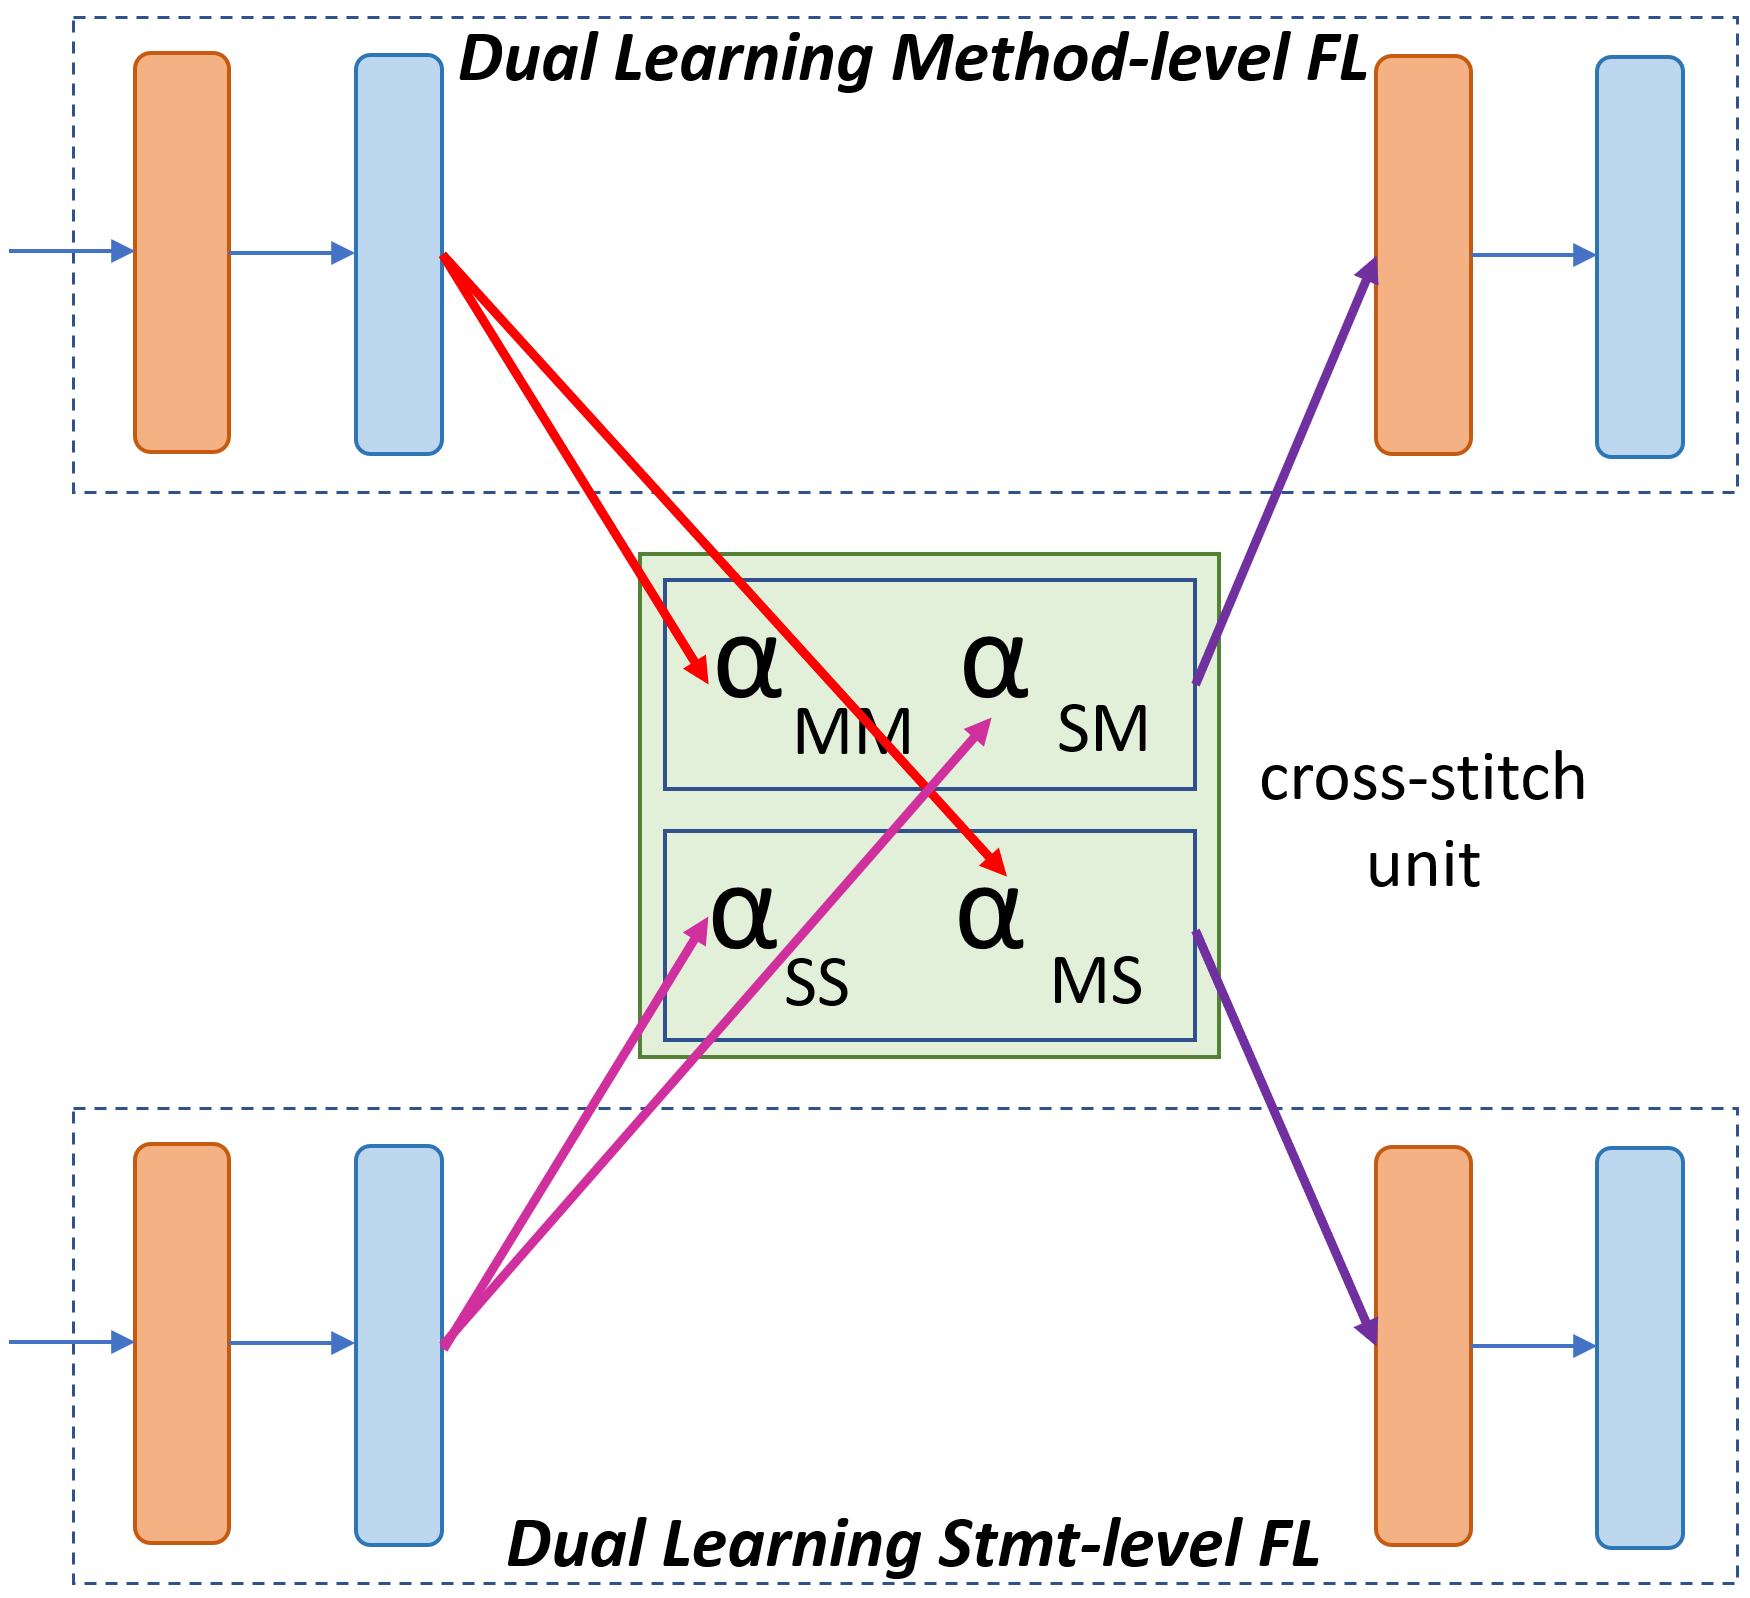
\includegraphics[width=2in]{graphs/cross-stitch.png}
	\caption{Dual Learning via Cross-stitch Unit}
	\label{cross-stitch}
\end{figure}

This section explains our dual learning scheme in step 3 (illustrated
in Figures~\ref{dual-learning} and~\ref{cross-stitch}). The input of
this step includes two feature graphs $G_M$ and $G_S$ for the method
and statement levels. Each node in each feature graph is a vector
computed for a method or a statement (explained in
Section~\ref{feature-learning:sec}). The output is the output graphs
for methods and statements. For the training process, each node in an
output graph has a buggy or non-buggy label.  For the prediction, each
node in an output graph will be predicted as buggy or non-buggy.

%After having the vectorized graph $G_m$ and $G_s$ for both the method-level and the statement-level features,

%in this step, \tool applies a dual learning fault localization model to extract the fault locations. So there are two main tasks in this step, including the method-level fault localization and the statement-level fault localization. So the input for this step is the two graphs $G_m$ and $G_s$, and the expected output is the prediction label for each node in these two graphs from these two tasks.

%Tien
\noindent {\bf Graph Convolution Network (GCN) for FL.} First, {\tool}
has two GCN models~\cite{kipf2016semi}, each for FL at the method and
statement levels. Each GCN model has $n-1$ pairs of a graph
convolution layer (\code{Conv}) and a rectified linear unit
(\code{ReLU}). They are aimed to consume and learn the characteristic
features in the input feature graph. The last pair of each GCN model
is a pair of a graph convolution layer (\code{Conv}) and a softmax
layer (\code{SoftMax}). The \code{SoftMax} layer plays the role of the
classifier on whether a node corresponding to a method or a statement
is labeled as buggy or non-buggy.

\noindent {\bf Dual Learning with Cross-stitch Unit.} In a regular GCN
model, those above pairs of \code{Conv} and \code{ReLU} are connected
to one another. However, to achieve dual learning between method-level
and state\-ment-level FL (\code{methFL} and \code{stmtFL}), we apply a
cross-stitch technique~\cite{misra2016cross} to connect the two GCN
models. The sharing of representations between \code{methFL} and
\code{stmtFL} is modeled by learning a linear combination of the input
features in both feature graphs. At each of the \code{ReLU} layer of
each GCN model (Figure~\ref{cross-stitch}), we aim to learn such a
linear combination of the output from the graph convolution layer
(\code{Conv}) of \code{methFL} and \code{stmtFL} models.

The top sub-network in Figure~\ref{dual-learning} gets direct
supervision from \code{methFL} and indirect supervision (through
cross-stitch units) from \code{stmtFL}~\cite{misra2016cross}.
Cross-stitch units help regularize both tasks \code{methFL} and
\code{stmtFL} by learning and enforcing shared representations by
combining feature maps~\cite{misra2016cross}.


%Tien
%The α values of a cross-stitch unit model linear combinations of
%feature maps. Their initialization in the range [0, 1] is important
%for stable learning, as it ensures that values in the output
%activation map (after cross-stitch unit) are of the same order of
%magnitude as the input values before linear combination.
%-----

\noindent {\bf Formulation.} Let us explain the mathematic foundation
of this scheme. For each pair of the GCN model, the outputs of the
\code{ReLU} layer, called the hidden states, are computed as follows:
\begin{equation}\label{eq:1}
	\hat{A} = D'^{-\frac{1}{2}}A'D'{-\frac{1}{2}}
\end{equation}

\begin{equation}\label{eq:2}
	H_i = \Delta(\hat{A}X_iW_i)
\end{equation}
Where $A'$ is the adjacency matrix of each feature graph; $D'$ is the
degree matrix; $W_i$ is the weight matrix for layer $i$; $X_i$ is the
input for layer $i$; $H_i$ is the hidden state of layer $i$; and
$\Delta$ is the activation function \code{ReLU}. $H_i$ is the output
from the \code{ReLU} layer. In a regular GCN, it is the input of the
next layer of GCN (i.e., the input of \code{Conv}).

In Figures~\ref{dual-learning} and~\ref{cross-stitch}, a cross-stitch
unit is inserted between the \code{ReLU} layer of the previous pair
and the \code{Conv} layer of the next one. The input of the
cross-stitch is the outputs of the two \code{ReLU} layers: $H_M^i$ and
$H_S^i$ (i.e., the hidden states of those layers at \code{methFL} and
\code{stmtFL}). We aim to learn the linear combinations of both inputs
of the cross-stitch unit, which is parameterized using the weights
$\alpha$.

The output of the cross-stitch unit is computed as:
\begin{equation}\label{cross-stitch-formula}
	\begin{bmatrix}
		X_M^{i+1}\\
		X_S^{i+1}
	\end{bmatrix}
        =
        \begin{bmatrix}
		\alpha_{MM} &  \alpha_{MS} \\
		\alpha_{SM} &  \alpha_{SS}
	\end{bmatrix}
	\begin{bmatrix}
		H_M^{i}\\
		H_S^{i}
	\end{bmatrix}
\end{equation}
Where $\alpha$ is the trainable weight matrix; $X_M^{i+1}$ and
$X_S^{i+1}$ are the inputs for the $(i+1)^{th}$ layers of GCN at the
method and statement levels.

$X_M^{i+1}$ and $X_S^{i+1}$ contain the information learned from both
\code{MethFL} and \code{StmtFL}, which helps achieve the main goal for
dual learning to enhance the performance of fault localization on both
levels.

In general, $\alpha$s can be set. If $\alpha_{MS}$ and $\alpha_{MS}$
are set to zeros, the layers are made to be task-specific.  The
$\alpha$ values model linear combinations of feature maps. Their
initialization in the range [0,1] is important for stable learning, as
it ensures that values in the output activation map (after
cross-stitch unit) are of the same order of magnitude as the input
values before linear combination~\cite{misra2016cross}.




%units combine the activations from multiple networks and can be
%trained end-to-end.

%Specifically, \tool firstly builds two separate GCN models \cite{kipf2016semi} for the method-level fault localization and the statement-level fault localization. For the GCN model applied on the method-level, there are $i$ graph convolutional layer $Conv_1, Conv_2, ..., Conv_i$ as shown in Figure \ref{dual-learning} and after each graph convolutional layer $Conv_i$, there is $ReLU$ layer follows it. Considering a graph convolutional layer $Conv_i$ and the following $ReLU$ layer together as one big layer, the GCN model contains $i$ layers in total. The only special case is in the last layer. There is a $SoftMax$ layer following the graph convolutional layer instead of a $RuLU$ layer. Similar to the GCN model applied on the method-level, for the statement-level fault location, there is the other GCN model with $i$ layers. Each layer contains one graph convolutional layer $Conv'_i$ and one $Relu$ layer. And the $SoftMax$ layer replaces the $ReLU$ layer in the last layer of the GCN model.


%To achieve the information sharing between two layers as a dual learning framework, we use the cross-stitch unit \cite{misra2016cross} for help. To be more detailed, for each layer of GCN, it calculates the hidden status using the following formula.





%Where $A'$ is the adjacency matrix; $D'$ is the degree matrix; $W_i$ is the weight matrix for layer $i$; $X_i$ is the input for layer $i$; $H_i$ is the hidden status of layer $i$; and $\Delta$ is the activation function $ReLU$. $H_i$ here is the output from the $ReLU$ layer and will be regarded as the input of the next layer of GCN. The cross-stitch unit is suitable to be added here.

%As seen in Figure \ref{dual-learning}, after the $ReLU$ layers we have $H_i^m$ and $H_i^s$ as the method-level and the statement-level hidden status. By putting them all into the cross-stitch unit, we have:

%\begin{equation}\label{eq:3}
%	\begin{bmatrix}
%		W_{m,m} &  W_{m,s} \\
%		W_{s,m} &  W_{s,s}
%	\end{bmatrix}
%	\begin{bmatrix}
%		H_m^{i}\\
%		H_s^{i}
%	\end{bmatrix}=
%	\begin{bmatrix}
%		X_m^{i+1}\\
%		X_s^{i+1}
%	\end{bmatrix}
%\end{equation}

%Where $W$ is the trainable or preset weight matrix, in \tool, we make it as the trainable weights; $X$ is the input for the $i+1$ layer of GCN. So with the cross-stitch unit, \tool gets $X_m^{i+1}$ and $X_s^{i+1}$ in this step as the input for the $i+1$ layer instead of directly feed $H_i^m$ and $H_i^s$ into the $i+1$ layer as input. The $X_m^{i+1}$ and $X_s^{i+1}$ contains the information learned from both the method-level and the statement-level that can help achieve the main goal for dual learning to enhance the performance of fault localization on both levels.

%But one special situation \tool may face in the cross-stitch unit is that the size of the outputs $H_i^m$ and $H_i^s$ from layer $i$ may be different. The different size of matrix will make the cross-stitch unit not work as expected.

If the sizes of the $H_M^{i}$ and $H_S^{i}$ are different, we need to adjust the sizes of the matrices. From Formula~\ref{cross-stitch-formula}, we have:
\begin{equation}\label{eq:4}
	X_M^{i+1} = \alpha_{MM}H_M^{i} + \alpha_{MS}H_S^{i}
\end{equation}
\begin{equation}\label{eq:5}
  X_S^{i+1} = \alpha_{SM}H_M^{i} + \alpha_{SS}H_S^{i}
\end{equation}

%Within formula \ref{eq:4} and \ref{eq:5}, \tool would like to resize $H_s^{i}$ in formula \ref{eq:4} and resize $H_m^{i}$ in formula \ref{eq:5}.

We resize $H_s^{i}$ in Formula~\ref{eq:4} and resize $H_m^{i}$ in
Formula~\ref{eq:5} if needed. We use the image processing technique {\em
  bilinear interpolation}. We pad zeros to the matrix to make the
aspect ratio 1:1. The bilinear interpolation is used for
resizing. If the size needs to be reduced, we do the center crop
on the matrix to match the required size.

{\tool} also has a trainable threshold for \code{SoftMax} to
 classify if a node corresponding to a method or a statement is buggy or not.

%By solving this problem, the cross-stitch unit can help share the information between two GCN models for both the method-level and the statement-level fault localization. The dual-learning fault localization model accepts the vectorized graphs as input and generates the label for each node. And there is a trainable threshold to determine if the node belongs to the $buggy$ class or the $non-buggy$ class. Thus, by collecting all nodes marked as $buggy$, \tool regards this set of predicted $buggy$ methods/statements as the output.

